\usepackage[a4paper,margin=24mm]{geometry}
\usepackage{amsmath,amssymb,amsthm,mathtools}
\usepackage{booktabs,longtable,array}
\usepackage{xcolor}
\usepackage{tikz}
\usetikzlibrary{arrows.meta,calc,positioning}
\usepackage[unicode,colorlinks,linkcolor=blue!45!black,urlcolor=blue!45!black]{hyperref}
\definecolor{ink}{HTML}{23354A}
\definecolor{mist}{HTML}{EAF0F5}
\definecolor{leaf}{HTML}{E9F3EF}
\definecolor{sand}{HTML}{F7F1E6}
\hypersetup{pdfauthor={Nil-Bohr Lean development},pdfsubject={Lean 4 formalization of the supplied manuscript}}
\setlength{\emergencystretch}{2em}
\raggedbottom
\newtheorem{theorem}{Theorem}
\newtheorem{proposition}[theorem]{Proposition}
\newtheorem{lemma}[theorem]{Lemma}
\newtheorem{corollary}[theorem]{Corollary}
\theoremstyle{definition}
\newtheorem{definition}[theorem]{Definition}
\newtheorem{remark}[theorem]{Remark}

\newcommand{\E}{\mathbb E}
\newcommand{\N}{\mathbb N}
\newcommand{\Z}{\mathbb Z}
\newcommand{\R}{\mathbb R}
\newcommand{\C}{\mathbb C}
\newcommand{\T}{\mathbb T}
\newcommand{\PP}{\mathbb P}
\newcommand{\one}{\mathbf 1}
\newcommand{\ee}{\mathrm e}
\newcommand{\Cramer}{\textup{Cr\'amer}}
\newcommand{\support}{\operatorname{supp}}
\newcommand{\abs}[1]{\lvert#1\rvert}
\newcommand{\norm}[1]{\lVert#1\rVert}
\newcommand{\tn}[1]{\norm{#1}_{\T}}
\newcommand{\code}[1]{\texttt{\detokenize{#1}}}
\newcommand{\source}[1]{\par\smallskip\noindent\textbf{Manuscript label.} \code{#1}\par\smallskip}
\newcommand{\openwork}{\par\smallskip\noindent\textbf{Lean status.} The full Lean proof remains open.\par}

% Upstream leanblueprint parses these commands in its web renderer.
% For PDF builds, validate all referenced labels and print Lean links.
\ExplSyntaxOn
\NewDocumentCommand{\uses}{m}
 {\clist_map_inline:nn {#1}{\vphantom{\ref{##1}}}\ignorespaces}
\NewDocumentCommand{\proves}{m}
 {\clist_map_inline:nn {#1}{\vphantom{\ref{##1}}}\ignorespaces}
\NewDocumentCommand{\lean}{m}
 {\par\smallskip\noindent\begingroup\normalfont\small\raggedright
  \textbf{Lean.}\space
  \clist_map_inline:nn {#1}{\nolinkurl{##1}\quad\allowbreak}
  \par\endgroup\smallskip}
\ExplSyntaxOff
\newcommand{\leanok}{}
\newcommand{\notready}{}
\newcommand{\printgraph}{\begin{center}
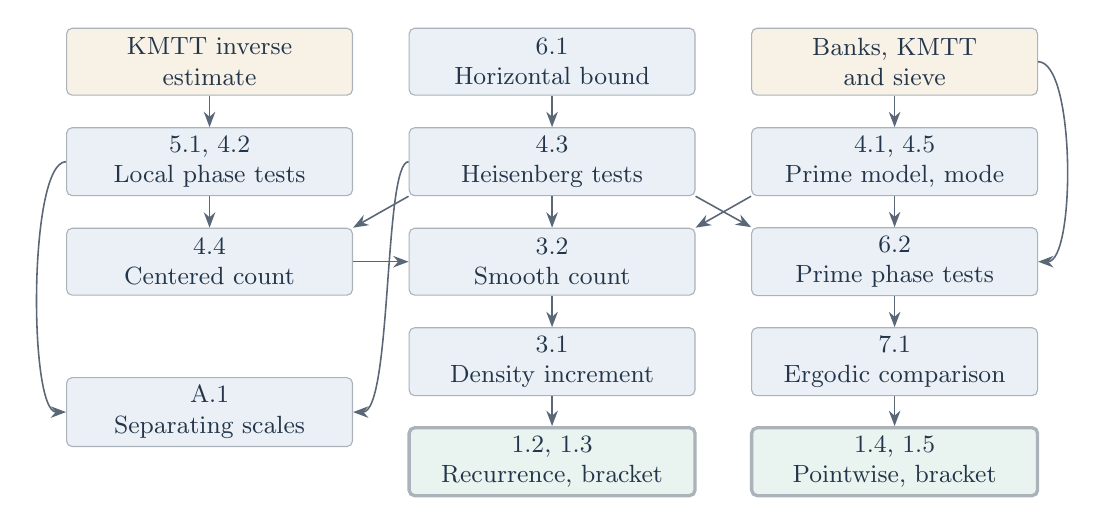
\begin{tikzpicture}[
  x=1cm,y=1cm, >=Stealth,
  stmt/.style={draw=ink!38,rounded corners=2pt,minimum height=0.85cm,text width=3.42cm,align=center,
     font=\small,inner sep=3pt,fill=mist,text=ink},
  ext/.style={stmt,fill=sand},
  conclusion/.style={stmt,fill=leaf,very thick},
  depends/.style={->,draw=ink!75,line width=0.57pt}]
  \node[ext] (inverse) at (-4.35,0) {KMTT inverse\\estimate};
  \node[stmt] (horizontal) at (0,0) {6.1\\Horizontal bound};
  \node[ext] (prime) at (4.35,0) {Banks, KMTT\\and sieve};
  \node[stmt] (local) at (-4.35,-1.27) {5.1, 4.2\\Local phase tests};
  \node[stmt] (phase) at (0,-1.27) {4.3\\Heisenberg tests};
  \node[stmt] (mult) at (4.35,-1.27) {4.1, 4.5\\Prime model, mode};
  \node[stmt] (bare) at (-4.35,-2.54) {4.4\\Centered count};
  \node[stmt] (compare) at (0,-2.54) {3.2\\Smooth count};
  \node[stmt] (weighted) at (4.35,-2.54) {6.2\\Prime phase tests};
  \node[stmt] (increment) at (0,-3.81) {3.1\\Density increment};
  \node[stmt] (erg) at (4.35,-3.81) {7.1\\Ergodic comparison};
  \node[conclusion] (rec) at (0,-5.08) {1.2, 1.3\\Recurrence, bracket};
  \node[conclusion] (pt) at (4.35,-5.08) {1.4, 1.5\\Pointwise, bracket};
  \node[stmt] (appendix) at (-4.35,-4.45) {A.1\\Separating scales};
  \draw[depends] (inverse) -- (local);
  \draw[depends] (horizontal) -- (phase);
  \draw[depends] (prime) -- (mult);
  \draw[depends] (local) -- (bare);
  \draw[depends] (phase.south west) -- (bare.north east);
  \draw[depends] (phase) -- (compare);
  \draw[depends] (phase.south east) -- (weighted.north west);
  \draw[depends] (mult.south west) -- (compare.north east);
  \draw[depends] (mult) -- (weighted);
  \draw[depends] (prime.east) .. controls (6.65,0) and (6.65,-2.54) .. (weighted.east);
  \draw[depends] (bare) -- (compare);
  \draw[depends] (compare) -- (increment);
  \draw[depends] (increment) -- (rec);
  \draw[depends] (weighted) -- (erg);
  \draw[depends] (erg) -- (pt);
  \draw[depends] (phase.west) .. controls (-2.14,-1.27) and (-2.03,-4.45) .. (appendix.east);
  \draw[depends] (local.west) .. controls (-6.65,-1.27) and (-6.65,-4.45) .. (appendix.west);
\end{tikzpicture}

\smallskip
\parbox{0.91\linewidth}{\small\raggedright
Arrows point from inputs to deductions. Shading denotes mathematical roles.
Quantitative Leibman enters 4.3. The KMTT inverse estimate also
gives the weak regularity used in 3.1. Ter\'av\'ainen enters 7.1.
The sieve inputs feed 6.2.
Mirek--Wan--Wright supplies the unrestricted pointwise limit. The prime
model and sieve supply prime normalization and the bracket boundary estimate.
Appendix A also uses the local multiplier. The comparison of bounds
uses the local estimate and Ter\'av\'ainen's fixed-family theorem.}
\end{center}
}
\newcommand{\printmapping}{\begin{longtable}{@{}l>{\raggedright\arraybackslash}p{0.46\linewidth}
  >{\raggedright\arraybackslash}p{0.38\linewidth}@{}}
\toprule
PDF & Source label & Mathematical role\\
\midrule
\endhead
Intro. & Unnumbered, source lines 212--231 &
  \hyperref[checked-intro-fast-obstruction]{Fast-approximation obstruction}\\
Intro. & Equation (7) and the quotient window &
  \hyperref[checked-heisenberg-window]{Open return window}\\
Intro. & Unnumbered, source lines 375--404 &
  \hyperref[checked-bohr-weights]{Pointwise Bohr weights}\\
Intro. & Unnumbered, source lines 406--422 &
  \hyperref[checked-bohr-eigenfunction]{Bohr eigenfunction example}\\
Intro. & Unnumbered, source lines 467--476 &
  \hyperref[checked-prime-progressions]{Progressions in selected primes}\\
Intro. & Unnumbered, source lines 478--482 &
  \hyperref[checked-maximal-domination]{Maximal domination}\\
Overview & Equation (10) and comparison in the surrounding text &
  \hyperref[checked-ambient-discrete]{Ambient counting comparison}\\
Overview & Unnumbered, source lines 542--559 &
  \hyperref[checked-ambient-norm]{Ambient Gowers obstructions}\\
1.1 & \code{c:bohr} & Finite Bohr restrictions\\
1.2 & \code{t:recurrence} & Quantitative recurrence\\
1.3 & \code{c:bracket-recurrence} & Bracket recurrence\\
1.4 & \code{t:pointwise} & Common pointwise limit and prime density\\
1.5 & \code{c:bracket-pointwise} & Bracket pointwise limit and density\\
1.6 & No source label &
  \hyperref[checked-smooth-factors]{Direct smooth-factor argument}\\
11--13 & \code{e:normalized-gowers}, \code{e:u-def}, \code{e:u-below-U} &
  \hyperref[checked-norm-foundations]{Interval and progression norms}\\
2.1 & \code{d:Cq} & Coefficient class\\
3.1 & \code{p:selected-density-increment} & One density increment\\
3.2 & \code{t:relative-selector-comparison} & Count comparison\\
4.1 & \code{p:high-order-relative-prime} & Prime weight replaced by $1$\\
4.2 & \code{t:main} & Local generalized von Neumann estimate\\
4.3 & \code{p:heisenberg-phase} & Scalar, twisted, and centered tests with
  \hyperref[checked-green-tao-adapter]{quantitative Leibman specialization}\\
4.4 & \code{l:unweighted-selector-relative-range} & Centered selector bounded on smooth moduli\\
4.5 & \code{l:vertical-mode-multiplier} & Localized vertical multiplier\\
5.1 & \code{p:localinverse} & Spatial local phase extraction\\
6.1 & \code{l:heisenberg-horizontal} & Horizontal Diophantine bound\\
44 & \code{e:phitildeonprog} &
  \hyperref[checked-twisted]{Uniform prefix bound for partial summation}\\
6.2 & \code{p:prime-phase} & Prime-weighted polynomial-phase bound\\
7.1 & \code{p:ergodic-comparison} & Smooth ergodic comparison\\
A.1 & \code{p:separating-family} & Dilation obstruction\\
App. A & Final paragraph & \hyperref[checked-iteration-moduli]{Sizes of admissible moduli}\\
\bottomrule
\end{longtable}
}
